\documentclass{templateNote}
\usepackage{tcolorbox}
\usepackage{hyperref}
\usepackage{amsmath}
\usepackage{amssymb}
\usepackage{soul}

\begin{document}

\imagenlogoU{img/logoNGMFormal_sinF.png}
\linklogoU{https://github.com/NicoGomezM} 
% \imagenlogoD{img/logo-ubb-txt-face.png} 
\titulo{Unidad 1}
\asignatura{Gestión Presupuestaria y Financiera}
\autor{
    \indent
    Nicolás {Gómez Morgado}
}


\portada
\margenes 
\tableofcontents
\newpage

\section{Conceptos clave}

\begin{itemize}
    \item \textbf{Presupuesto:} Es un plan financiero que detalla los ingresos y gastos de una organización en un periodo de tiempo determinado.
    \item \textbf{Pronostico de ventas:} Es una estimación de las ventas futuras de una empresa.
    \item \textbf{Estados financieros:} Son informes que presentan la situación financiera y los resultados de las operaciones de una empresa.
    \item \textbf{Estados financieros proyectados:} Son estados financieros que se proyectan en el futuro.
    \item \textbf{Bonos y acciones:} Son instrumentos financieros que permiten a las empresas obtener financiamiento.
    \item \textbf{Valor par, valor sobre la par y valor:} Son conceptos relacionados con el valor de los bonos.
    \item \textbf{Acciones preferentes:} Son acciones que tienen preferencia en el pago de dividendos.
    \item \textbf{Dividendos:} Son pagos que las empresas hacen a sus accionistas.
    \item \textbf{Autofinanciación:} Es la capacidad de una empresa para financiar sus operaciones con sus propios recursos.
    \item \textbf{Activo financiero:} Es un instrumento financiero que representa un derecho de propiedad sobre un activo. Esta determinado por:
    \begin{itemize}
        \item Utilidad que genera en el futuro.
        \item La tasa de interés.
    \end{itemize}
    \item \textbf{Valor del dinero:} Cambia con el tiempo, por lo que un peso hoy vale más que un peso en el futuro. Se debe distinguir entre:
    \begin{itemize}
        \item Valor nominal (¿Cuanto dinero hay?)
        \item Valor real (¿Cuanto se puede comprar con ese dinero?) 
    \end{itemize}
    \item \textbf{Criterio por decision:} Depende de la rentabilidad del proyecto.
    \item \textbf{Riesgo:} Es la probabilidad de que un proyecto no se desarrolle como se espera.
    \item \textbf{Rentabilidad del proyecto:} Lo que el proyecto puede o va a generar con mi inversion inicial.
\end{itemize}

\section{Tipos de intereses}
\subsection{Interés simple}
\noindent El interés simple es aquel que se calcula sobre el capital inicial, sin importar si se reinvierte o no. Algunas de las características del interés simple son:
\begin{itemize}
    \item El capital inicial se mantiene constante durante toda la operación.
    \item El interés siempre es el mismo para cualquier periodo de la operación.
    \item La tasa de interés solo se aplica al capital inicial.
\end{itemize}

\begin{tcolorbox}[colback=blue!10!white,colframe=blue!60!black,title=Ejemplo]
    \begin{enumerate}
        \item Si invierto \$10.000.000 a una tasa de interés simple del 15\% anual, ¿cuánto dinero tendré al cabo de 3 años?
    \end{enumerate}
    \textbf{Formula:}
    \begin{align*}
        VF &= VP(1 + i \cdot n)
    \end{align*}
    $VF$ = Valor futuro\\
    $VP$ = Valor presente\\
    $i$ = Tasa de interés\\
    $n$ = Número de periodos\\
    \textbf{Solución:}\\
    \begin{minipage}{0.5\textwidth}
        \begin{align*}
            \textit{Datos:} \quad
            VP &= \$10.000.000\\
            i &= 0.15\\
            n &= 3
        \end{align*}
    \end{minipage}
    \begin{minipage}{0.5\textwidth}
        \begin{align*}
            VF &= VP(1 + i \cdot n)\\
            VF &= \$10.000.000(1 + 0.15 \cdot 3)\\
            VF &= \$10.000.000(1 + 0.45)\\
            VF &= \$10.000.000(1.45)\\
            VF &= \$14.500.000
        \end{align*}
    \end{minipage}
    \center Por lo tanto genere \$4.500.000 en intereses.
\end{tcolorbox}


\subsection{Interés compuesto}
\noindent El interés compuesto es aquel que se calcula sobre el capital inicial y los intereses generados en periodos anteriores. Algunas de las características del interés compuesto son:
\begin{itemize}
    \item El capital inicial aumenta en cada periodo de la operación debido a que se suman los intereses.
    \item La tasa de interés se aplica sobre un capital que va variando.
    \item Los intereses aumentan en relación con el tiempo.
\end{itemize}

\begin{tcolorbox}[colback=blue!10!white,colframe=blue!60!black,title=Ejemplo]
    \begin{enumerate}
        \item Si invierto \$10.000.000 a una tasa de interés compuesto del 15\% anual, ¿cuánto dinero tendré al cabo de 3 años?
    \end{enumerate}
    \textbf{Formula:}
    \begin{align*}
        VF &= VP(1 + i)^n
    \end{align*}
    $VF$ = Valor futuro\\
    $VP$ = Valor presente\\
    $i$ = Tasa de interés\\
    $n$ = Número de periodos\\
    \textbf{Solución:}\\
    \begin{minipage}{0.5\textwidth}
        \begin{align*}
            \textit{Datos:} \quad
            VP &= \$10.000.000\\
            i &= 0.15\\
            n &= 3
        \end{align*}
    \end{minipage}
    \begin{minipage}{0.5\textwidth}
        \begin{align*}
            VF &= VP(1 + i)^n\\
            VF &= \$10.000.000(1 + 0.15)^3\\
            VF &= \$10.000.000(1.15)^3\\
            VF &= \$10.000.000(1.520875)\\
            VF &= \$15.208.750
        \end{align*}
    \end{minipage}
    \center Por lo tanto genere \$5.208.750 en intereses.
\end{tcolorbox}
\newpage

\section{Costos de oportunidad}
\noindent El costo de oportunidad es el valor de la mejor opción que se deja de lado al tomar una decisión.
\subsection{Criterios de decision}
\begin{center}
    \begin{itemize}
        \item Rentabilidad del proyecto > Costo de oportunidad $\Rightarrow$ \textbf{Proyecto Rentable}.
        \item Rentabilidad del proyecto < Costo de oportunidad $\Rightarrow$ \textbf{Proyecto no Rentable}.
        \item Rentabilidad del proyecto = Costo de oportunidad $\Rightarrow$ \textbf{Proyecto Indiferente}.
    \end{itemize}        
\end{center}
\begin{figure}[H]
    \centering
    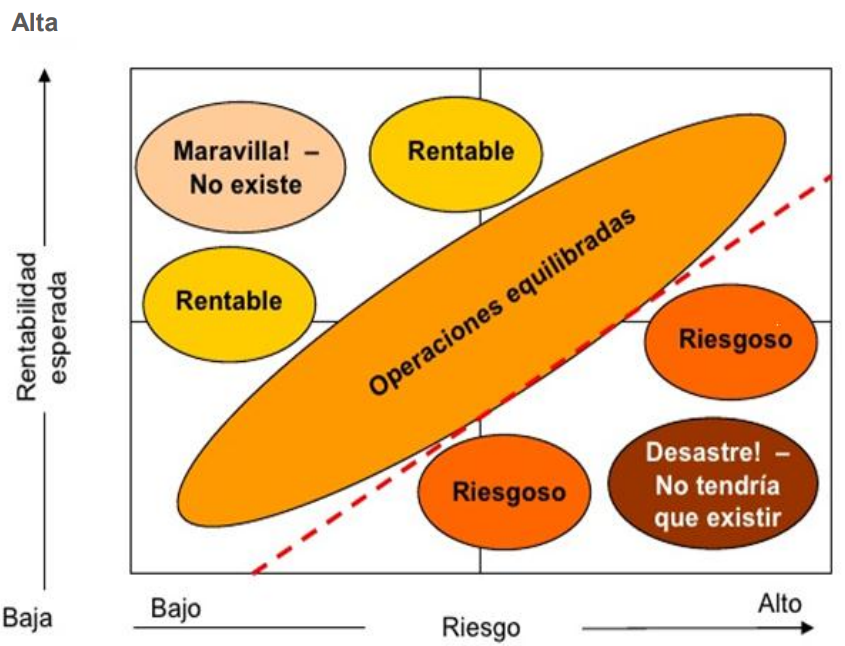
\includegraphics[height=8cm]{img/costosOport.png}
    \caption{Figura representativa criterios}
\end{figure}
\newpage

\section{Valor del dinero y Tasas de rendimiento}
\subsection{Tasa de rendimiento}
\noindent La tasa de rendimiento es la rentabilidad que se obtiene de una inversión. Se puede calcular mediante la siguiente formula:
\begin{align*}
    \textnormal{Rendimiento} &= \frac{\textnormal{Ganancia}}{\textnormal{Inversion}} \cdot 100\%
\end{align*}

\subsection{Valor futuro (VF)}
\noindent Valor que tendrá una inversión en el futuro tomando en cuenta un capital inicial (VP), una tasa de interés (i) y un número de periodos (n). Se puede calcular mediante la siguiente formula:
\begin{align*}
    VF &= VP(1 + i)^n
\end{align*}
\textit{Donde:}
\begin{align*}
    VF &= \textnormal{Valor futuro}\\
    VP &= \textnormal{Valor presente}\\
    i &= \textnormal{Tasa de interés}\\
    n &= \textnormal{Número de periodos}\\
\end{align*} 

\subsection{Valor presente (VP)}
\noindent Valor que tiene una inversión en el presente tomando en cuenta un capital futuro (VF), una tasa de interés (i) y un número de periodos (n). Se puede calcular mediante la siguiente formula:
\begin{align*}
    VP &= \frac{VF}{(1 + i)^n}
\end{align*}
\textit{Donde:}
\begin{align*}
    VF &= \textnormal{Valor futuro}\\
    VP &= \textnormal{Valor presente}\\
    i &= \textnormal{Tasa de interés}\\
    n &= \textnormal{Número de periodos}\\
\end{align*}

\begin{tcolorbox}[colback=blue!10!white,colframe=blue!60!black,title=Ejemplo]
    \noindent Usted estima que al realizar un proyecto, en una año podrá venderlo en \$420.000.000. Para lo anterior, usted necesita invertir \$370.000.000. Adicionalmente usted cree que el proyecto es tan 
    riesgoso como una inversion en el mercado de valores que le ofrece un rendimiento esperado del 12\%. \\\\
    \textit{Datos:}
    \begin{align*}
        VF &= \$420.000.000\\
        VP &= \$370.000.000\\
        n &= 1
    \end{align*}
    \begin{enumerate}
        \item Calcule el valor presente del activo (Considere una tasa de interés del 5\%).
        \begin{align*}
            VP &= \frac{VF}{(1 + i)^n}\\
            VP &= \frac{\$420.000.000}{(1 + 0.05)^1}\\
            VP &= \frac{\$420.000.000}{1.05}\\
            VP &= \$400.000.000
        \end{align*}
        \item Calcule el rendimiento del activo.
        \begin{align*}
            \textnormal{Rendimiento} &= \frac{\textnormal{Ganancia}}{\textnormal{Inversion}} \cdot 100\%\\
            \textnormal{Rendimiento} &= \frac{\$420.000.000 - \$370.000.000}{\$370.000.000} \cdot 100\%\\
            \textnormal{Rendimiento} &= \frac{\$50.000.000}{\$370.000.000} \cdot 100\%\\
            \textnormal{Rendimiento} &= 13.51\%\\
            \textnormal{Rendimiento} &\approx 14\% 
        \end{align*}
        \item ¿Cual seria el costo de oportunidad?\\
        \noindent El costo de oportunidad es el valor de la mejor opción que se deja de lado al tomar una decisión. En este caso, el costo de oportunidad es el rendimiento esperado del mercado de valores, que es del 12\%.
        \item ¿Realizaría la inversion?\\
        \noindent Si, ya que la rentabilidad del proyecto es mayor al costo de oportunidad ($\textnormal{Rendimiento} > \textnormal{Costo de Oprtunidad} \rightarrow $ 14\% > 12\%).
    \end{enumerate}
\end{tcolorbox}

\subsection{Valuación de flujos de efectivo en varios periodos}
\subsubsection{Flujo de efectivo descontado(FED)} 
\noindent Calculo del valor presente tomando en cuenta varias cantidades de dinero en diferentes periodos. Se calcula mediante la siguiente formula:
\begin{align*}
    FED &= \sum_{t=1}^{n} \frac{{\textnormal{VF}}_t}{(1 + i)^t}
\end{align*}
\textit{Donde:}
\begin{align*}
    FED &= \textnormal{Flujo de efectivo descontado}\\
    \textnormal{VF}_t &= \textnormal{Valor futuro en el periodo t}\\
    i &= \textnormal{Tasa de interés}\\
    n &= \textnormal{Número de periodos}\\
\end{align*}

\subsubsection{Valor actual Neto (VAN/VNA/VPN)}
\noindent Son los flujos de efectivo descontados menos la inversión inicial, el cual si posee un valor positivo, el proyecto es rentable. Se calcula mediante la siguiente formula:
\begin{align*}
    VAN &= {\sum_{t=1}^{n} \frac{{\textnormal{VF}}_t}{(1 + i)^t}} - \textnormal{Inversion} \\
    VAN &= FED - \textnormal{Inversion}
\end{align*}
\textbf{Consideraciones del VAN:}
\begin{itemize}
    \item Si el VAN $> 0$, el proyecto crea valor.
    \item Si el VAN $< 0$, el proyecto destruye valor.
    \item Si el VAN $= 0$, el proyecto esta en un punto de equilibrio.
\end{itemize}

\begin{tcolorbox}[colback=blue!10!white,colframe=blue!60!black,title=Ejemplo]
    \noindent Calcular el valor actual neto de un proyecto que tiene una inversión inicial de \$2.000 y los siguientes flujos de efectivo:
    \begin{minipage}{0.5\textwidth}
        \centering
        \begin{tabular}{|c|c|}
            \hline
            \multicolumn{2}{|c|}{\textbf{Datos}} \\ \hline
            $i$ & 10\% \\ \hline
            $n$ & 4 \\ \hline
            Inversion & \$2.000 \\ \hline
        \end{tabular}
    \end{minipage}
    \begin{minipage}{0.5\textwidth}
        \centering
        \begin{tabular}{|c|c|c|c|}
            \hline
            \multicolumn{4}{|c|}{\textbf{Detalle de flujos}} \\ \hline
            Año 1 & Año 2 & Año 3 & Año 4 \\ \hline
            800 & 600 & 400 & 900 \\ \hline
        \end{tabular}
    \end{minipage}

    \begin{align*}
        VAN &= \sum_{t=1}^{n} \frac{{\textnormal{VF}}_t}{(1 + i)^t} - \textnormal{Inversion}\\
        VAN &= \frac{800}{(1 + 0.10)^1} + \frac{600}{(1 + 0.10)^2} + \frac{400}{(1 + 0.10)^3} + \frac{900}{(1 + 0.10)^4} - 2000\\
        VAN &= \frac{800}{1.10} + \frac{600}{1.21} + \frac{400}{1.331} + \frac{900}{1.4641} - 2000\\
        VAN &= 727.27 + 495.87 + 300.67 + 614.52 - 2000\\
        VAN &= 2138.33 - 2000\\
        VAN &= 138.33 \\
        VAN &\approx 138
    \end{align*}
    \center Por lo tanto el proyecto crea valor y es rentable.
\end{tcolorbox}    

\textbf{Inconvenientes del VAN:}
\begin{itemize}
    \item No toma en cuenta el cambio del valor del dinero en el tiempo causado por la inflación y tipos de interés.
    \item No toma en cuenta los ingresos después del plazo de recuperación, lo que puede llevar a decisiones erróneas como priorizar inversiones de corto plazo o con altos flujos de caja iniciales.
    \item Necesita de una prevision de flujos de caja futuros (estimar los gastos o ingresos en caja), lo que puede llevar a errores en la estimación.
    \item Prioriza los proyectos que permiten recuperar la inversion inicial en corto plazo antes que los que pueden generan mayor rentabilidad a largo plazo.
\end{itemize}

\subsection{Tasa interna de retorno}
\noindent Tasa de descuento en la cual el VAN el igual a cero. Se calcula mediante la siguiente formula:
\begin{align*}
    VAN &= \sum_{t=1}^{n} \frac{{\textnormal{VF}}_t}{(1 + \textnormal{\hl{TIR}})^t} - \textnormal{Inversion} = 0\\
    \textnormal{\hl{TIR}} &= \% 
\end{align*}

\begin{tcolorbox}[colback=blue!10!white,colframe=blue!60!black,title=Ejemplo]

    \begin{minipage}{0.5\textwidth}
        \centering
        \begin{tabular}{|c|}
            \hline
            \multicolumn{1}{|c|}{\textbf{TIR}} \\ \hline
            13\% \\ \hline
        \end{tabular}
    \end{minipage}
    \begin{minipage}{0.5\textwidth}
        \centering
        \begin{tabular}{|c|c|}
            \hline
            \multicolumn{2}{|c|}{\textbf{Datos}} \\ \hline
            $i$ & 10\% \\ \hline
            $n$ & 4 \\ \hline
            Inversion & \$2.000 \\ \hline
        \end{tabular}
    \end{minipage}

    \begin{align*}
        VAN &= \sum_{t=1}^{n} \frac{{\textnormal{VF}}_t}{(1 + \textnormal{{TIR}})^t} - \textnormal{Inversion} \\
        VAN &= -2000 + \frac{800}{(1 + 0.13)^1} + \frac{600}{(1 + 0.13)^2} + \frac{400}{(1 + 0.13)^3} + \frac{900}{(1 + 0.13)^4} \\
        VAN &= -2000 + 707 + 468 + 276 + 549\\
    \end{align*}

\end{tcolorbox}
\newpage

\section{\hl{Amortización}}
\noindent Pago gradual de deuda en un periodo de tiempo determinado por medio de una deuda a través de una cuota con interés fijo. La cuota se puede calcular mediante la siguiente formula:
\begin{align*}
    \textnormal{Cuota} &= \textnormal{Crédito} \cdot \frac{i\%}{1-((1+i\%)^{-n})}
\end{align*}
\begin{figure}[H]
    \centering
    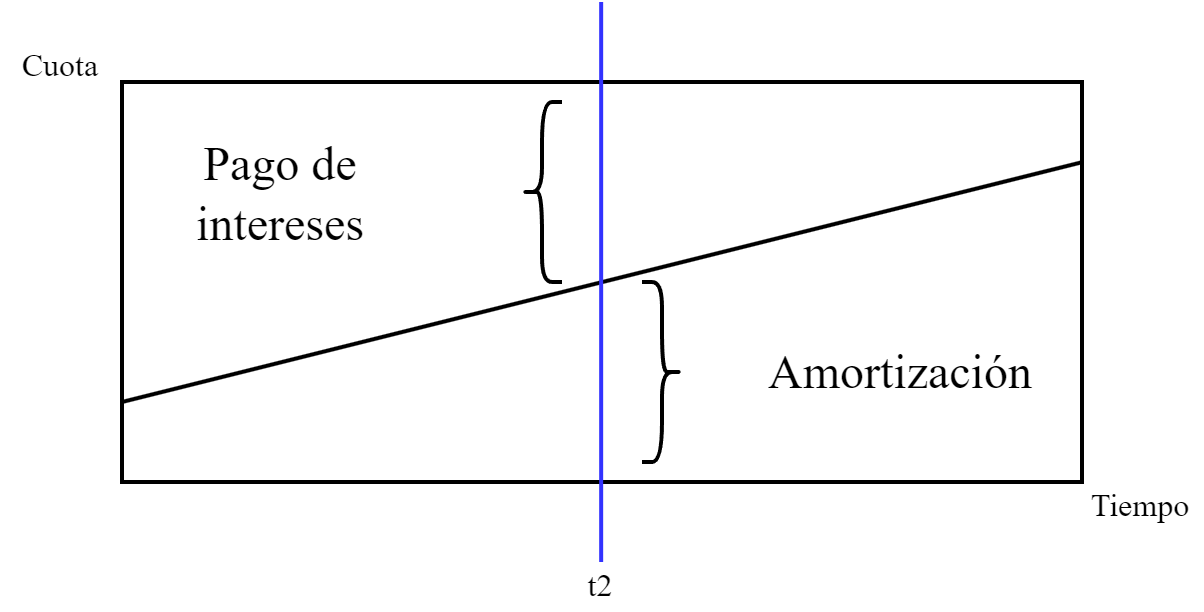
\includegraphics[height=5.5cm]{img/amortiz.png}
\end{figure}

\begin{tcolorbox}[colback=orange!10!white,colframe=orange!60!black,title=Observación]
    En un momento determinado yo debo la deuda original menos lo amortizado.
\end{tcolorbox}
\newpage

\section{Tasa de interés equivalente}
\noindent Si se tiene una tasa de interés anual $ia$; la tasa de interés mensual se puede calcular mediante la siguiente formula:
\begin{align*}
    \textnormal{Con interés compuesto: }im &= ((1 + ia)^{\frac{1}{12}} - 1) \cdot 100\%\\
\end{align*}

\begin{tcolorbox}[colback=blue!10!white,colframe=blue!60!black,title=Ejecicios]
    \begin{itemize}
        \item Interés anual = 15\% $\Rightarrow$ Interés mensual = 1.17\%
        \item Interés anual = 9\% $\Rightarrow$ Interés mensual = 0.72\%
    \end{itemize}
\end{tcolorbox}

\begin{tcolorbox}[colback=orange!10!white,colframe=orange!60!black,title=Observación]
    Recordar que interés compuesto es aquel que se calcula sobre el capital inicial y los intereses generados en periodos anteriores.
\end{tcolorbox}

\section{Carga anual equivalente (CAE)}
\begin{itemize}
    \item El CAE es un indicador \textbf{porcentual}, que incluye los intereses, gastos y seguros asociados al crédito, expresados en forma anual que 
        permiten hacer una comparación objetiva del costo del crédito entre las entidades.
    \item Mediante el CAE, las personas pueden comparar diferentes alternativas de crédito, sin importar las variables establecidas por cada entidad.
    \item Un CAE bajo indica que el crédito es más barato, ya que considera todos los elementos del crédito.
\end{itemize}
\noindent El CAE por ley debe ser entregado por todas las entidades financieras que otorgan créditos de consumo. Se puede calcular mediante la siguiente formula:
\begin{align*}
    CAE &= (1+i_f)^n - 1
\end{align*}
\textit{Donde:}
\begin{align*}
    i_f &= \textnormal{Tasa de interés efectiva}\\
    n &= \textnormal{Número de periodos}
\end{align*}
\newpage

\section{Análisis financiero}
\noindent \textbf{Objetivos:} Determinar el diagnóstico a corto plazo de una organización, determinando fortalezas y debilidades (como en un FODA) 
    financieras, para una oportuna y eficaz toma de decisiones.\\ 
\begin{itemize}
    \item Elementos de diagnostico a corto plazo
    \item Administración empresa privada (\textit{enfoque de la carrera})
    \item Análisis financiero se compara al análisis de muestra de sangre.
\end{itemize}

\subsection{Objetivos de un buen gerente de finanzas}
\begin{itemize}
    \item Maximizar rentabilidad (\textit{acorde al marco valórico}) a los dueños (\textit{personas/acciones}) del capital.
    \item Crecimiento estable de la empresa a largo plazo. (\textit{Tasa de crecimiento nulo, no estable; Tasa de crecimiento inestable, mal gerente})
    \item Cumplimiento con valores estratégicos de la empresa.
    \item Mercado sensible y castiga ante cualquier daño de imagen de una empresa.
\end{itemize}

\subsection{Estructura del balance}
\begin{figure}[H]
    \centering
    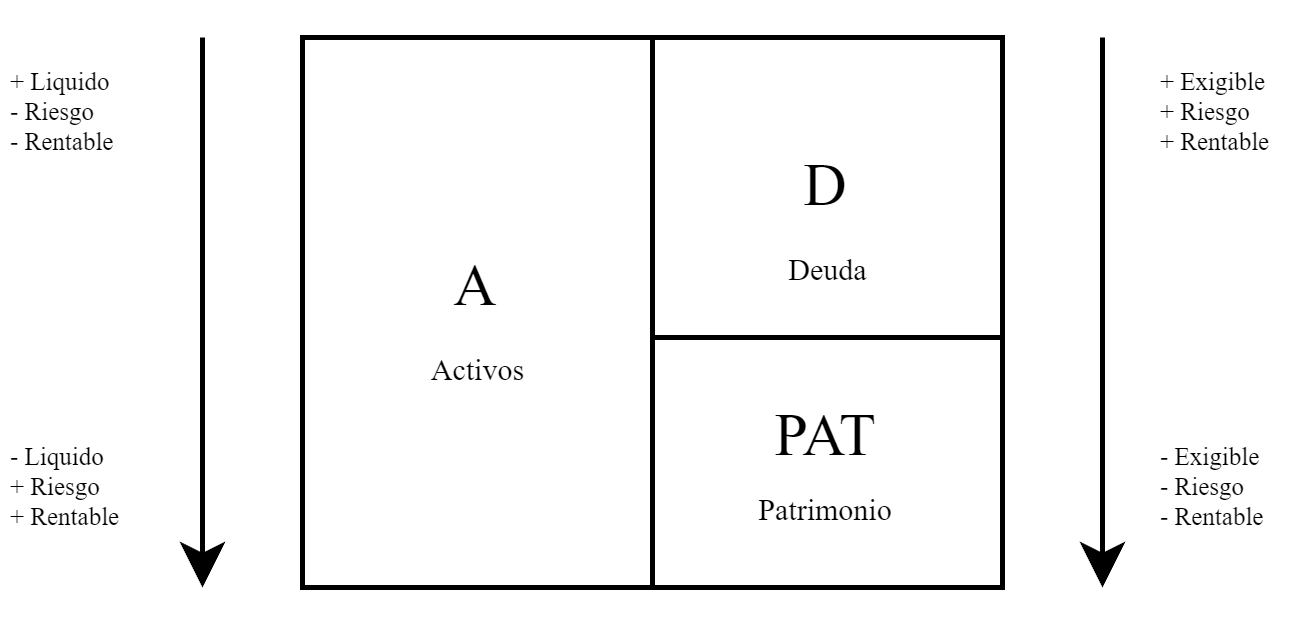
\includegraphics[height=7.5cm]{img/estrucBalance.png}
\end{figure}
\newpage

\section{Capital neto del trabajo (CNT)}
\noindent El capital neto de trabajo es un indicador financiero que mide la capacidad de una empresa para cumplir con sus obligaciones a corto plazo. Se define como la \textbf{diferencia entre los activos circulantes y los pasivos de corto plazo} por lo tanto se calcula de la siguiente forma:
\begin{align*}
    CNT &= AC - PCP
\end{align*}
\textit{Donde:}
\begin{align*}
    CNT &= \textnormal{Capital neto de trabajo}\\
    AC &= \textnormal{Activos circulantes}\\
    PCP &= \textnormal{Pasivos corto plazo}
\end{align*}

\subsection{Activos circundantes}
\noindent Algunos tipos de activos circulantes son:
\begin{itemize}
    \item Efectivo en cajas y bancos.
    \item Inversiones temporales en instrumentos financieros.
    \item Cuentas por cobrar.
    \item Inventarios (materia prima, proceso y terminado).
\end{itemize}
\textbf{Característica:} Fácil conversión en efectivo en un plazo máximo de un año. 

\subsection{Pasivos de corto plazo}
\noindent Algunos tipos de pasivos de corto plazo son:
\begin{itemize}
    \item Proveedores.
    \item Cuentas por pagar.
    \item Impuestos por pagar. 
    \item Créditos menores o iguales a un año.
\end{itemize}
\textbf{Característica:} Deben ser cancelados en un plazo máximo de un año.

\subsection{Políticas del capital del trabajo}
\noindent Decisiones básicas enfocadas en el manejo eficiente de los recursos, nivel de inversion deseado (AC) y forma de financiamiento (PCP). Existen 3 tipos de políticas para \textbf{gestionar el capital de trabajo}:
\begin{itemize}
    \item \textbf{Política relajada:} A mayor capital de trabajo, menor riesgo de ser técnicamente insolvente.
    \item \textbf{Política restringida:} A menor capital de trabajo, mayor riesgo de ser técnicamente insolvente.
    \item \textbf{Política moderada:} Equilibrio entre riesgo y rentabilidad.
\end{itemize}

\subsubsection{Politica relajada}
\begin{itemize}
    \item Mantenimiento de saldos elevados en efectivo e inversiones temporales.
    \item Créditos flexibles, lo que resulta en un alto nivel de cuentas por cobrar.
    \item Grandes inversiones en inventarios.
    \item Mas financiamiento en el largo plazo, menor rendimiento (mayor gasto financiero en la manutención de la política) y menor riesgo (decisiones mas pensadas en un mayor plazo). 
\end{itemize}

\begin{figure}[H]
    \centering
    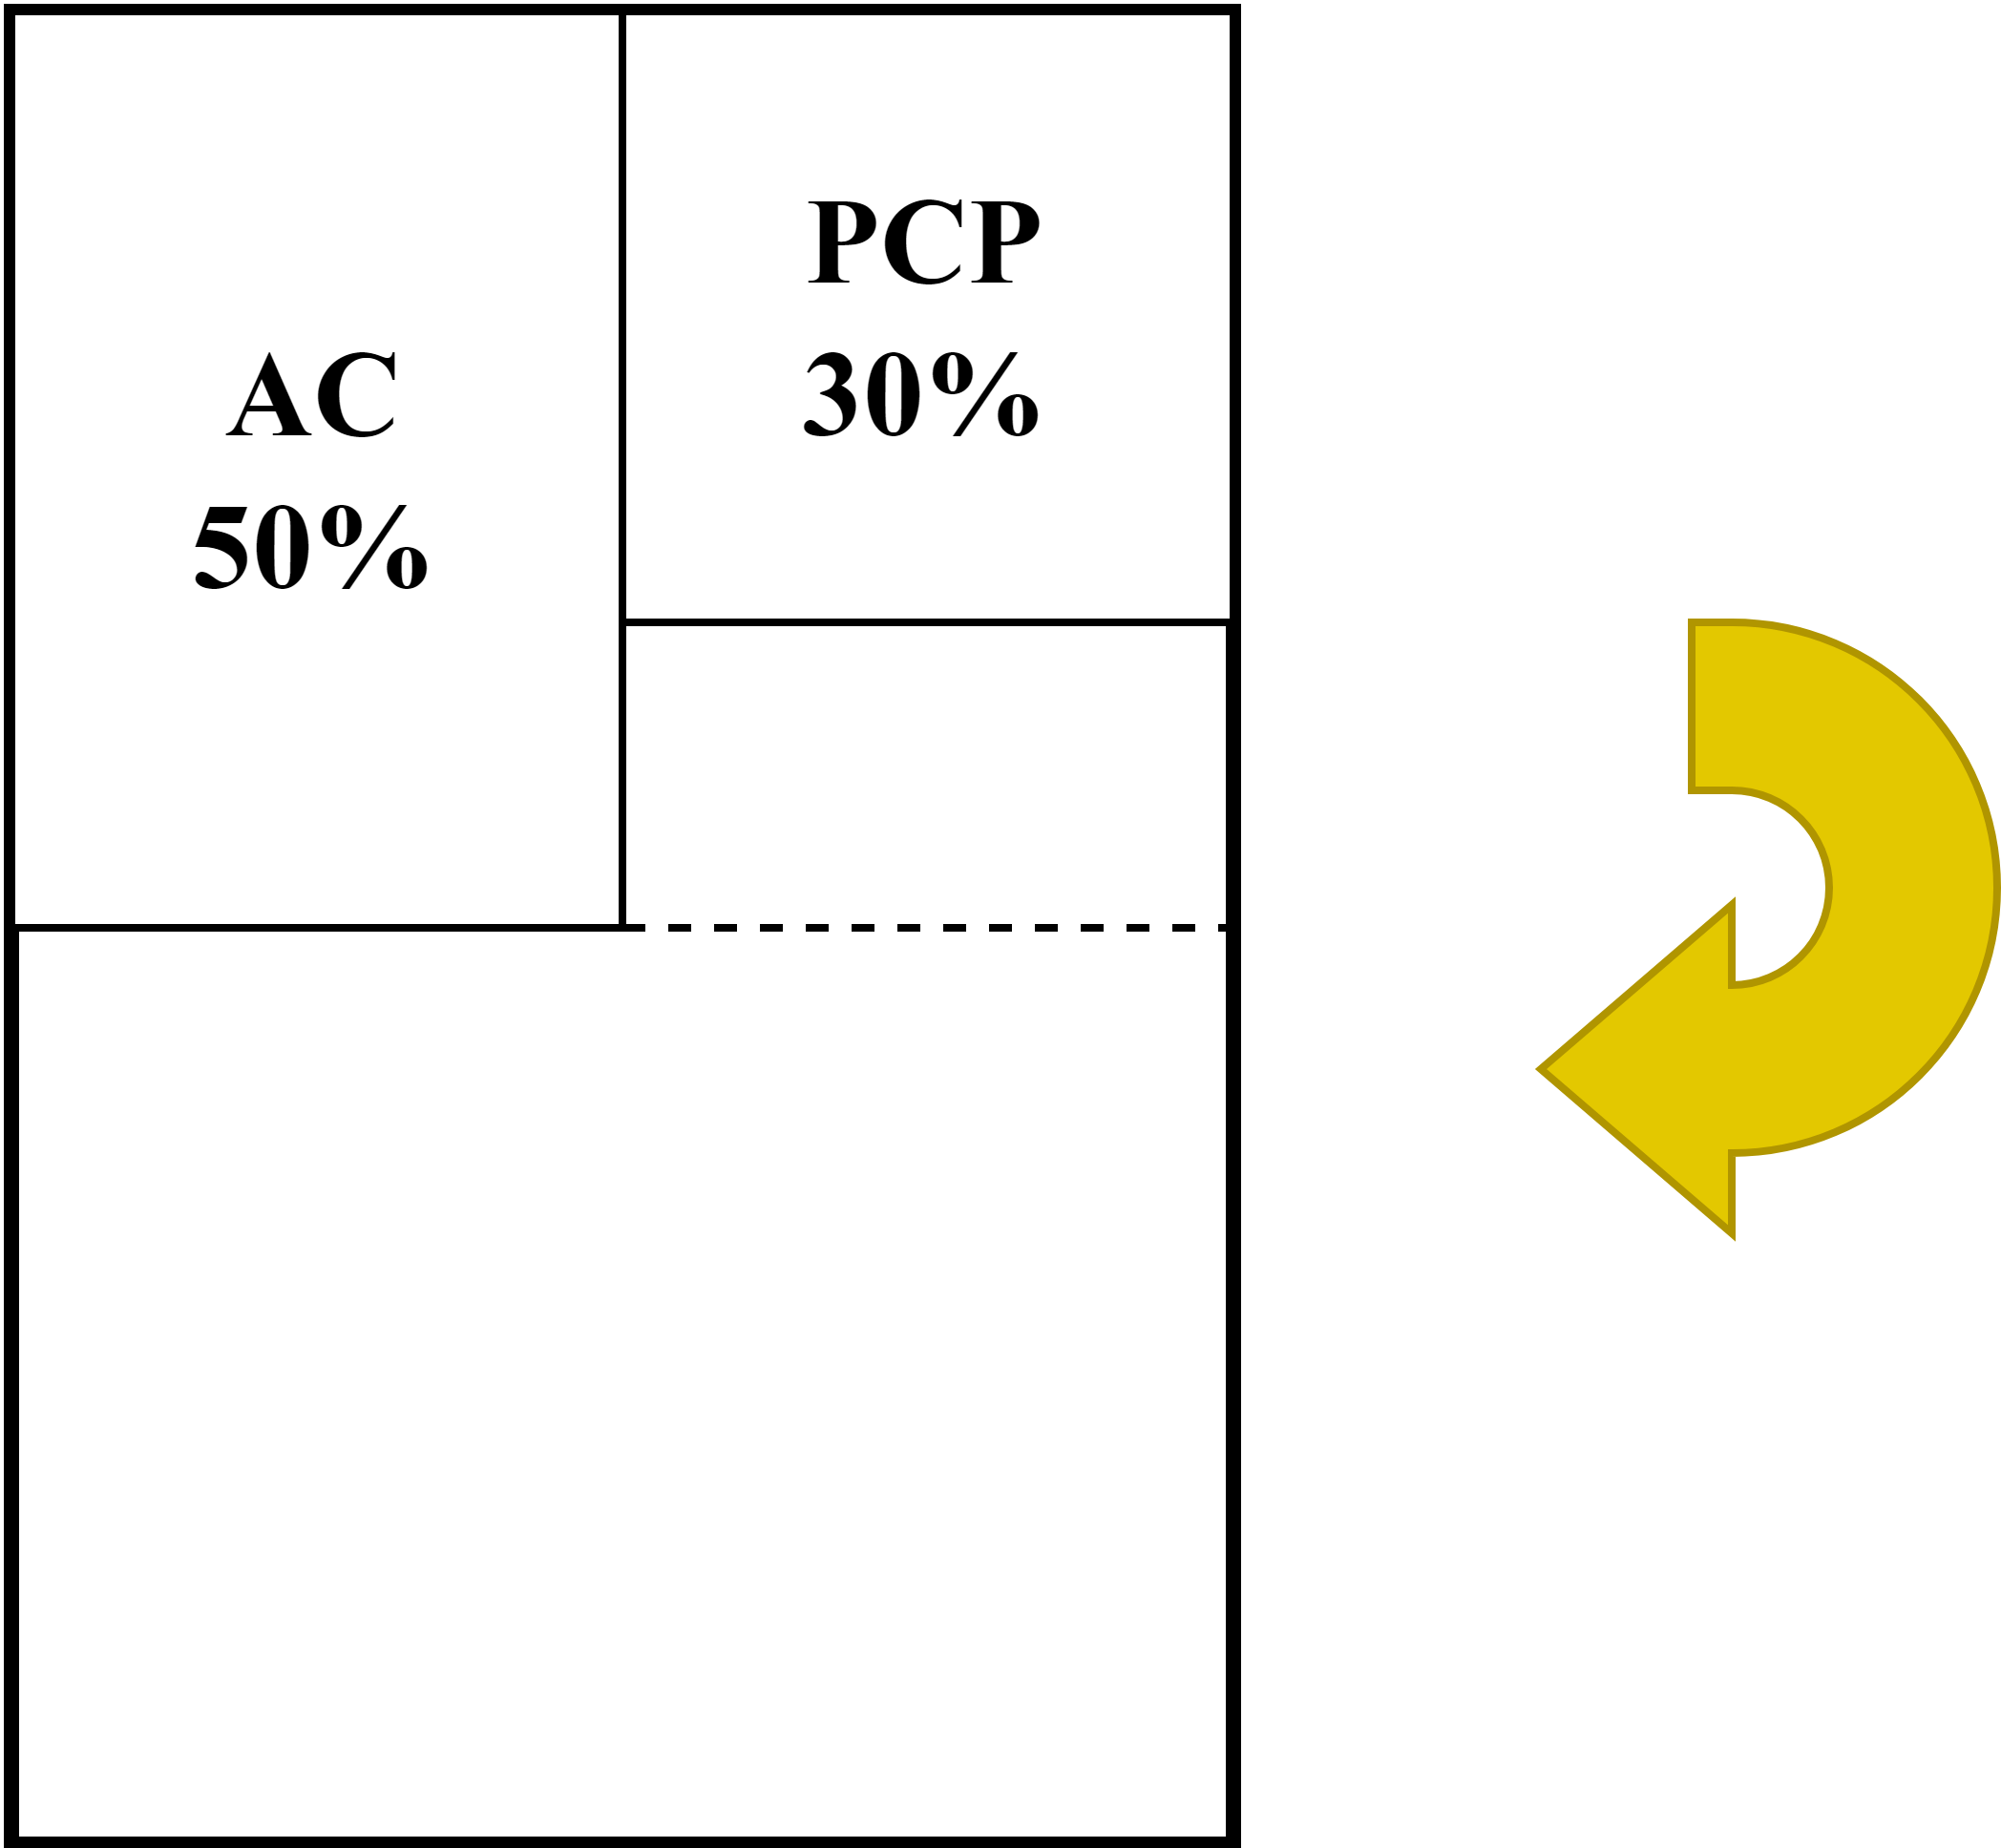
\includegraphics[height=3.5cm]{img/polirelajada.png}
\end{figure}

\subsubsection{Politica restringida}
\begin{itemize}
    \item Manejar poco efectivo y no invertir en valores temporales.
    \item Otorgar créditos solo a individuos selectos, provocando una disminución en cuentas por cobrar.
    \item Inversiones pequeñas en inventario, trabajar con mínimos.
    \item Mas financiamiento en el corto plazo, mayor rendimiento (menor gasto financiero en la manutención de la política) y mayor riesgo (decisiones mas rápidas en un menor plazo).
\end{itemize}
\begin{figure}[H]
    \centering
    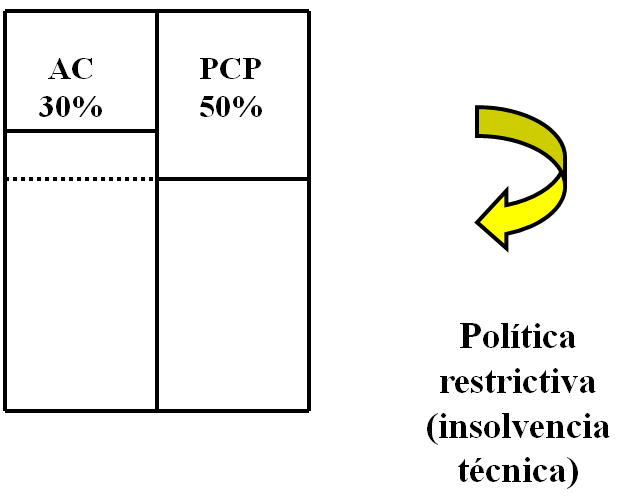
\includegraphics[height=3.5cm]{img/polirestrict.png}
\end{figure}
\newpage

\section{Análisis de indicadores}
\subsection{Análisis vertical}
\noindent El análisis vertical es una técnica que permite comparar los componentes de un estado financiero con un total, el cual se representa en porcentajes.
\textbf{Tipos de indicadores:}
\begin{enumerate}
    \item Índices de liquidez.
    \item Índices de actividad y rotación.
    \item Índices de endeudamiento.
    \item Índices de rentabilidad.
\end{enumerate}

\subsubsection{Índices de liquidez}
\noindent Capacidad de una empresa de convertir sus activos en caja o de obtener caja para satisfacer su pasivo circulante. Es decir, miden la solvencia de una empresa en el corto plazo.

\begin{tcolorbox}[colback=orange!10!white,colframe=orange!60!black,title=Observación]
    \textit{\textbf{Mientras mayores sean los índices de liquidez, mayor será la solvencia de la empresa en el corto plazo.-}}
\end{tcolorbox}

\begin{itemize}
    \item \textbf{Índice de liquidez corriente:} 
\end{itemize}

\end{document}